\documentclass[a4paper,11pt,titlepage]{article}

\usepackage[breaklinks=true]{hyperref}

\usepackage{pdflscape}

% encoding
\usepackage[utf8]{inputenc}
\usepackage[T1]{fontenc}

%Collaboration management
\usepackage[final,english]{fixme}
%read-me: http://mirrors.dotsrc.org/ctan/macros/latex/contrib/fixme/fixme.pdf

% layout
\bibliographystyle{ieeetr}

\usepackage[margin=3cm]{geometry}
\usepackage{textcomp}

% appearance
\usepackage{graphicx} 
\usepackage{color}

% math extensions
\usepackage{amsmath}
\usepackage{amssymb}
\usepackage{amsthm}
\usepackage{listings}

\lstset{%
  frame=trBL,
  frameround=fttt,
  basicstyle=\footnotesize\tt,
  keywordstyle=\bf,
  language = C,
  tabsize=2
}
\newcommand{\for}{\text{ for }}
\newcommand{\then}{\rightarrow}
\newcommand{\id}[1]{\ensuremath{\mathop{\mathit{#1}}\nolimits}}

% header and footer
\usepackage{fancyhdr}

\definecolor{qstgray}{gray}{0.9}
\makeatletter
\newenvironment{qst}{
  \begin{lrbox}{\@tempboxa}
    \begin{minipage}{\columnwidth}
      \footnotesize \slshape
    }
    {
    \end{minipage}
  \end{lrbox}
  \colorbox{qstgray}{\usebox{\@tempboxa}}
}
\makeatother

\fancypagestyle{fncy}{
  \lhead{\thecourse}
  \chead{\today}
  \rhead{Handin 2}
  \lfoot{}
  \cfoot{}
  \rfoot{\thepage}
  \renewcommand{\headrulewidth}{0.5pt}
  \renewcommand{\footrulewidth}{0.5pt}
}

\setcounter{secnumdepth}{2}
\setcounter{tocdepth}{2}

%\pagestyle{fncy} can't be used with progress 

% title
\title{\thecourse \\ \thetitle} 
\date{\today} 
\author{%
  \begin{tabular}{ll}
    Frederik Mogensen & 20080923\\
    Allan Stisen & 20083311\\
    Lasse Højgaard & 20080848
  \end{tabular}
}



\newcommand{\thecourse}{Wireless Sensor Networks}
\newcommand{\thetitle}{Mini-project 3 - Temperature sensing} 
\newcommand{\subsubsubsection}[1]{\underline{#1}\newline}

\begin{document}

\maketitle
\newpage

\tableofcontents
\newpage
\section{Project Description}


\begin{frame}
\frametitle{Description}

\begin{itemize}
	\item make a  sensor network which can measure the temperature periodically
	\item Sensor mote transmit results to sink
	\item Sensor shows the results by either:
	\begin{itemize}
		\item a blue ($\leq 15^{\circ} C $) led
		\item or a red $>15^{\circ} C$ led 
	\end{itemize}
	\item Sink sends ACK to sensor mote if receives package
	\item Sensor mote goes to sleep if receives ACK or try to retransmit $N$ times.
\end{itemize}
\end{frame}

\begin{frame}
\frametitle{Extensions of project}
\begin{description}
\item[Multiple motes] If there are multiple sensing motes, they send their sensing data to the sink.
\item[Plotting] Plot temperature vs. time (offline /online)
\item[Temperature average] The sink averages the temperature from the sensors.
\item[Temperature average sensor] The sensor motes averages $n$ temperatures before sending to the sink to improve energy efficiency of the application.

\end{description}
\end{frame}

%%% Local Variables: 
%%% mode: latex
%%% TeX-master: "../presentation"
%%% End: 

\section{Project implementation}


\begin{frame}
\frametitle{Project overview}
\begin{figure}[htbp]
   \centering
   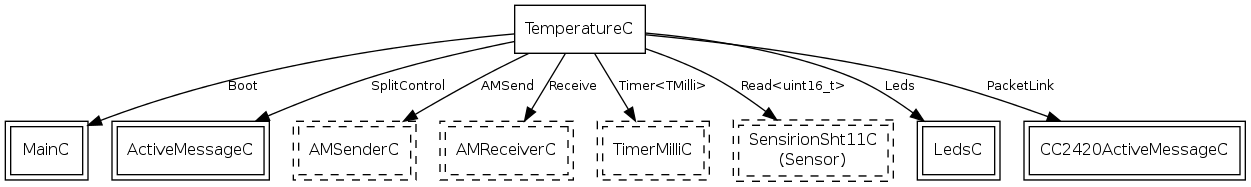
\includegraphics[width=\textwidth]{img/TemperatureAppC.png} 
\end{figure}

\end{frame}

\begin{frame}
\frametitle{Temperature measuring}
The conversion given a digital readout ($SO_{T}$) to a temperature value is given at the following formula:
\begin{align*}
	T &= d_{1} + d_{2} \cdot SO_{T}
\end{align*}
where the coefficients is the following
\begin{table}[ht]
\centering
\begin{tabular}{ | l | c | r | }
	\hline
	VDD & $d_{1} \ ^{\circ}  C$ & $d_{1} \ ^{\circ}  F$ \\
	\hline \hline
	5V & -40.1 & -40.2 \\
	\hline
	4V & -39.8 & -39.6 \\
	\hline
	3.5V & -39.7 & -39.5 \\
	\hline
	3V & -39.6 & -39.3 \\
	\hline
	2.5V & -39.4 & -38.9 \\
	\hline
\end{tabular}
\begin{tabular}{ | l | c | r | }
	\hline
	$SO_{T}$ & $d_{2}  \ ^{\circ}C$ & $d_{2} \ ^{\circ} F$ \\
	\hline \hline
	14 bit & 0.01 & 0.018 \\
	\hline
	12 bit & 0.04 & 0.072\\
	\hline
\end{tabular}
\caption{Temperature conversion coefficients}
\label{table:temperature}
\end{table}

\end{frame}

\begin{frame}[fragile]
\frametitle{Package ACK with PacketAcknowledgements interface}
\begin{lstlisting}[caption={TemperatureAppC.nc}]
 TemperatureC.PacketAcknowledgements -> ActiveMessageC;
\end{lstlisting}


\begin{lstlisting}[caption={TemperatureC.nc $\rightarrow$ sendReadings()}]
memcpy(call AMSend.getPayload(&sendBuf, sizeof(local)),
    &local, sizeof local);
call PacketAcknowledgements.requestAck(&sendBuf);
if (call AMSend.send(SINK_NR, &sendBuf, sizeof local)
    == SUCCESS) {
    sendBusy = TRUE;
    ackTries++;
}
\end{lstlisting}

\end{frame}

\begin{frame}[fragile]
\frametitle{Package ACK with PacketAcknowledgements interface}

\begin{lstlisting}[caption={TemperatureC.nc $\rightarrow$ AMSend.sendDone()}]
if(call PacketAcknowledgements.wasAcked(msg)) {
    reportSent();
    ackTries = 0;
} else {
    if (ackTries < NACKTRIES) {
        sendReadings();
    } else if (ackTries == NACKTRIES) {
        ackTries = 0;
        sleep();
    }
}
\end{lstlisting}

\end{frame}

\begin{frame}[fragile]
\frametitle{Package ACK with PacketLink interface}
\begin{lstlisting}[caption={TemperatureAppC.nc}]
TemperatureC.PacketLink -> CC2420ActiveMessageC;
\end{lstlisting}

\begin{lstlisting}[caption={TemperatureC.nc $\rightarrow$ sendReadings()}]
memcpy(call AMSend.getPayload(&sendBuf, sizeof(local)),
    &local, sizeof local);
call PacketLink.setRetries(&sendBuf, 10);
call PacketLink.setRetryDelay(&sendBuf, 500);
if (call AMSend.send(SINK_NR, &sendBuf, sizeof local)
    == SUCCESS) {
    sendBusy = TRUE;
}
\end{lstlisting}

\end{frame}

\begin{frame}[fragile]
\frametitle{Package ACK with PacketLink interface}

\begin{lstlisting}[caption={TemperatureC.nc $\rightarrow$ AMSend.sendDone()}]
if (call PacketLink.wasDelivered(msg)){
    reportSent();
    sleep();
} else {
    reportProblem();
    sleep();
}
\end{lstlisting}

\end{frame}

%%% Local Variables: 
%%% mode: latex
%%% TeX-master: "../presentation"
%%% End: 

\section{Project results}


\begin{frame}
\frametitle{Project results}
 
\end{frame}


\newpage
\bibliography{references}
\end{document}
